\chapter{Mengenal Kecerdasan Buatan dan Scikit-Learn}

\section{Teori}
Praktek teori penunjang yang dikerjakan :
\begin{enumerate}
\item
Definisi, Sejarah dan perkembangan Kecerdasan Buatan.

	\begin{enumerate}
		\item Definisi Kecerdasan Buatan
		\newline Kecerdasan Buatan (Artificial Intelligence) merupakan cabang ilmu dalam bidang komputer untuk mensimulasikan atau memodelkan kecerdasan manusia ke dalam komputer atau mesin yang bertujuan untuk memungkinkan suatu sistem berpikir layaknya seperti manusia.
		
		\item Sejarah dan Perkembangan Kecerdasan Buatan
		\newline Awal mula terbentuknya kecerdasan buatan dimulai pada tahun 1950-an oleh ilmuwan matematika bernama Alan Turing. Pada saat itu, Alan Turing dalam tulisannya yang berjudul "Computing Machinery and Intelligence" memberikan pernyataan yang membangkitkan semangat para ilmuwan dalam pengembangan Artificial Intelligence. Pada tahun 1956, Artifical Intelligence pertama kali muncul berkat adanya sebuah program AI Darthmouth Summer Research Project on Artificial Intelligence (DSRPAI). Melalui program tersebut menjadi awal mula perkembangan Artificial Intelligence hingga saat ini.
		\newline Pada tahun 1960-an, perkembangan AI menjadi cukup pesat, dimana pada saat itu komputer sudah mulai dapat menampung informasi yang cukup banyak dan dapat diakses dengan mudah. Pada saat itu juga, algoritma machine learning yaitu NLP (Natural Language Processing) mulai digunakan untuk memecahkan permasalahan sistem sehingga pemerintah mulai yakin dan mendukung mengenai perkembangan AI ini.Pada tahun 1970-an, Jepang telah berhasil menciptakan robot pertama yang mampu melihat, bergerak, dan berbicara. Hal tersebut membuat pemerintah dan korporat mulai yakin untuk berinvestasi pada perkembangan AI ini. Namun pada tahun 1973-1970 menjadi masa kelam perkembangan AI. Pada saat itu, para peneliti tidak dapat memenuhi target pengembangan AI mereka dikarenakan sistem komputer yang belum cukup canggih untuk memproses data dalam jumlah masif.	
		\newline Pada tahun 1990, menjadi kebangkitan dalam pengembangan AI, dimana pada saat itu mulai banyak diciptakannya robot-robot yang bisa berinteraksi dengan manusia seperti Deep Blue, Furby, dan RoBOT (AIBO). Memasuki abad 21 dan seiring perkembangan teknologi komputer yang mulai canggih, perkembangan AI menjadi semakin pesat. Banyak perusahaan teknologi yang mulai menggunakan dan mengembangkan AI untuk digunakan dikehidupan sehari-hari. Perkembangan AI kedepannya pasti akan semakin canggih dan akan banyak kemungkinan yang terjadi diluar bayangan kita saat ini. 
		
	\end{enumerate}
\item
Definisi Supervised Learning, Klasifikasi, Regresi dan Unsupervised Learning. Data set, Training Set dan Testing Set.

	\begin{enumerate}
		\item Supervised Learning
		\newline Supervised Learning adalah pendekatan yang ditentukan dengan menggunakan traning set  atau labeled set untuk membuat model yang  dapat meningkatkan akurasi dari waktu ke waktu. Dengan kata lain, semakin banyak model memproses data,  semakin akurat pemrosesan tersebut.
		
		\item Unsupervised Learning
		\newline Unsupervised Learning merupakan suatu pendekatan yang ditentukan dengan berdasarkan penggunaan traning set yang tidak berlabel. Pendekatan ini digunakan untuk menganalisa dan juga mengelompokan kumpulan data yang tidak berlabel. Selain itu, juga digunakan untuk menarik kesimpulan dari dataset dan mempelajari suatu data berdasarkan kedekatannya (clustering).
		
		\item Klasifikasi
		\newline Klasifikasi adalah suatu teknik yang digunakan untuk melakukan identifikasi beberapa data yang belum memiliki label untuk dikategorikan menjadi sebuah bagian dari kelas. 
		
		\item Regresi
		\newline Regresi adalah suatu teknik yang digunakan untuk mendefinisikan hubungan antara satu variabel dengan variabel lain. Teknik ini bertujuan untuk menemukan suatu fungsi yang dapat memodelkan data dengan meminimalkan error atau selisih nilai prediksi dengan nilai aslinya.
		
		\item Data Set
		\newline Data set adalah kumpulan informasi-informasi yang dijadikan satu kesatuan dan dapat dikelola sehingga menjadi sebuah data atau informasi baru. 
		
		\item Training Set
		\newline Training set merupakan bagian dari dataset yang digunakan untuk melatih algoritma agar mampu memprediksi atau menjalankan fungsi dari algoritma tersebut.
		
		\item Testing Set
		\newline Testing set merupakan bagian dari data set yang digunakan untuk mengetahui akurasi dan performa dari algoritma yang sudah di latih oleh training set sebelumnya.
		 
	\end{enumerate}
\end{enumerate}

\newpage
\section{Instalasi}
Membuka https://scikit-learn.org/stable/tutorial/basic/tutorial.html. Dengan menggunakan bahasa yang mudah dimengerti dan bebas plagiat. 
Dan wajib skrinsut dari komputer sendiri.
\begin{enumerate}
\item
Instalasi library scikit dari anaconda, mencoba kompilasi dan uji coba ambil contoh kode dan lihat variabel explorer.
		\begin{figure}[!htbp]
			\centering
			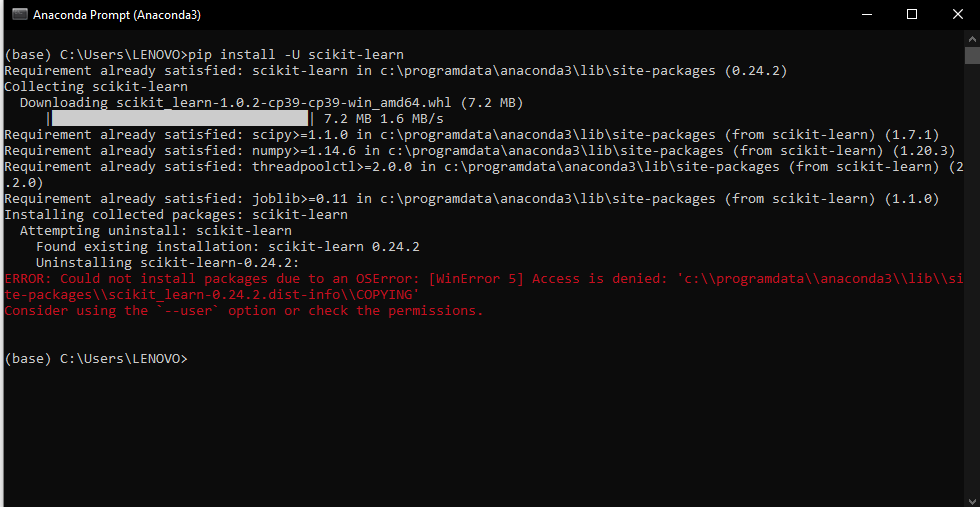
\includegraphics[scale=0.3]{figures/1.1.PNG}
			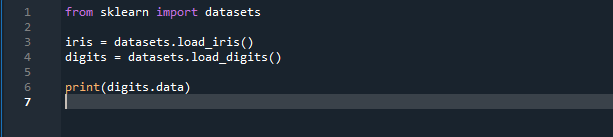
\includegraphics[scale=0.5]{figures/1.2.PNG}
			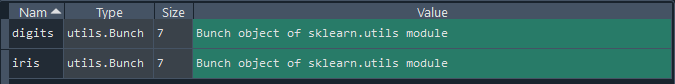
\includegraphics[scale=0.4]{figures/1.3.PNG}
		\end{figure}
	
\item
Mencoba Loading an example dataset, menjelaskan maksud dari tulisan tersebut dan mengartikan per baris.
		\begin{figure}[!htbp]
			\centering
			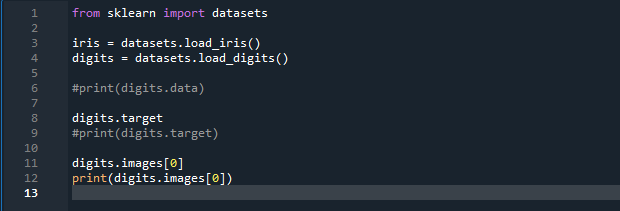
\includegraphics[scale=0.4]{figures/2.1.PNG}
			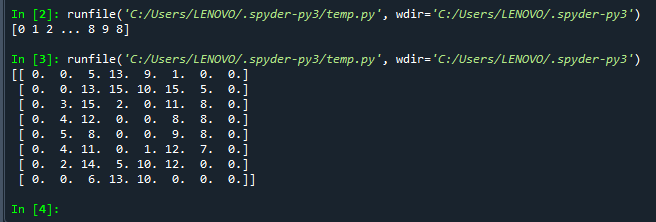
\includegraphics[scale=0.5]{figures/2.2.PNG}
		\end{figure}
\newpage
\item
Mencoba Learning and predicting, menjelaskan maksud dari tulisan tersebut dan mengartikan per baris.
		\begin{figure}[!htbp]
			\centering
			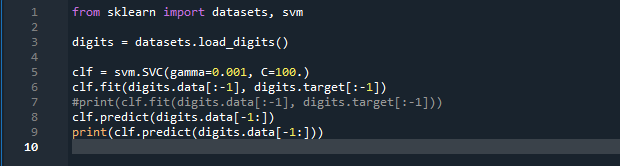
\includegraphics[scale=0.4]{figures/3.1.PNG}
			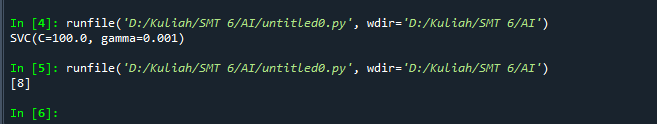
\includegraphics[scale=0.5]{figures/3.2.PNG}
		\end{figure}
\item
mencoba Model persistence, menjelaskan maksud dari tulisan tersebut dan mengartikan per baris.
		\begin{figure}[!htbp]
			\centering
			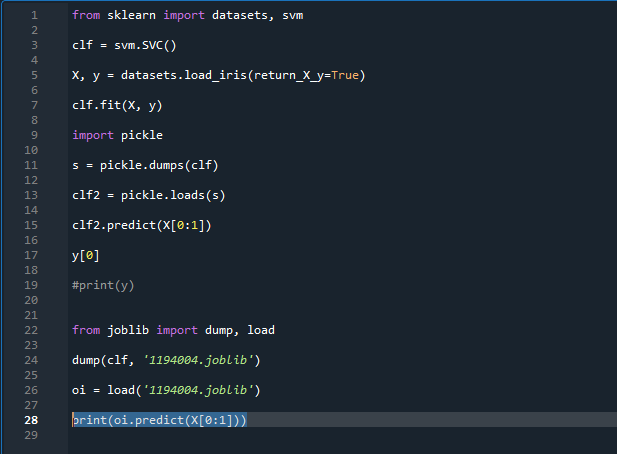
\includegraphics[scale=0.5]{figures/4.1.PNG}
			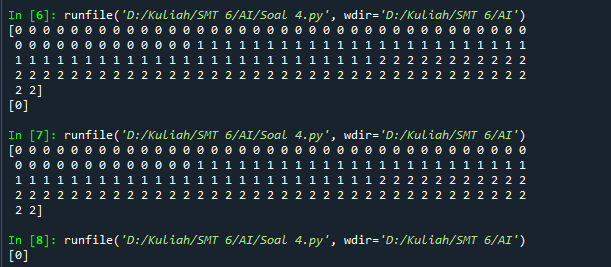
\includegraphics[scale=0.5]{figures/4.2.PNG}
		\end{figure}
\item 
Mencoba Conventions, menjelaskan maksud dari tulisan tersebut dan mengartikan per baris.
		\begin{figure}[!htbp]
			\centering
			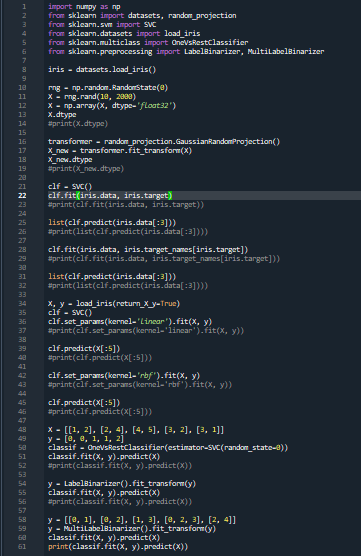
\includegraphics[scale=0.6]{figures/5.1.PNG}
			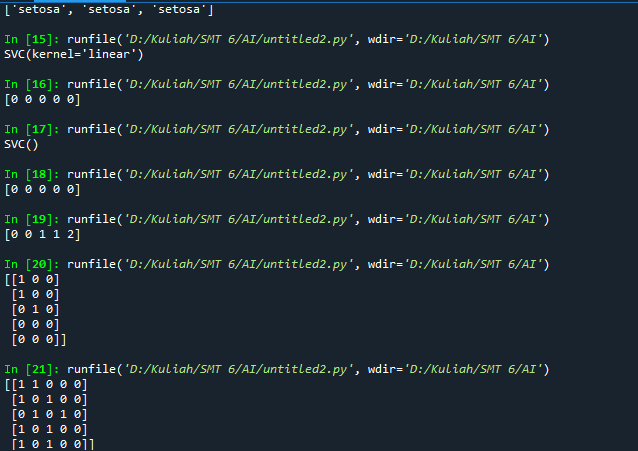
\includegraphics[scale=0.6]{figures/5.2.PNG}
		\end{figure}
\end{enumerate}

\newpage
\section{Penanganan Error}
Dari percobaan yang dilakukan di atas, apabila mendapatkan error maka:

\begin{enumerate}
	\item
	Screenshoot error.
	\begin{figure}[!htbp]
		\centering
		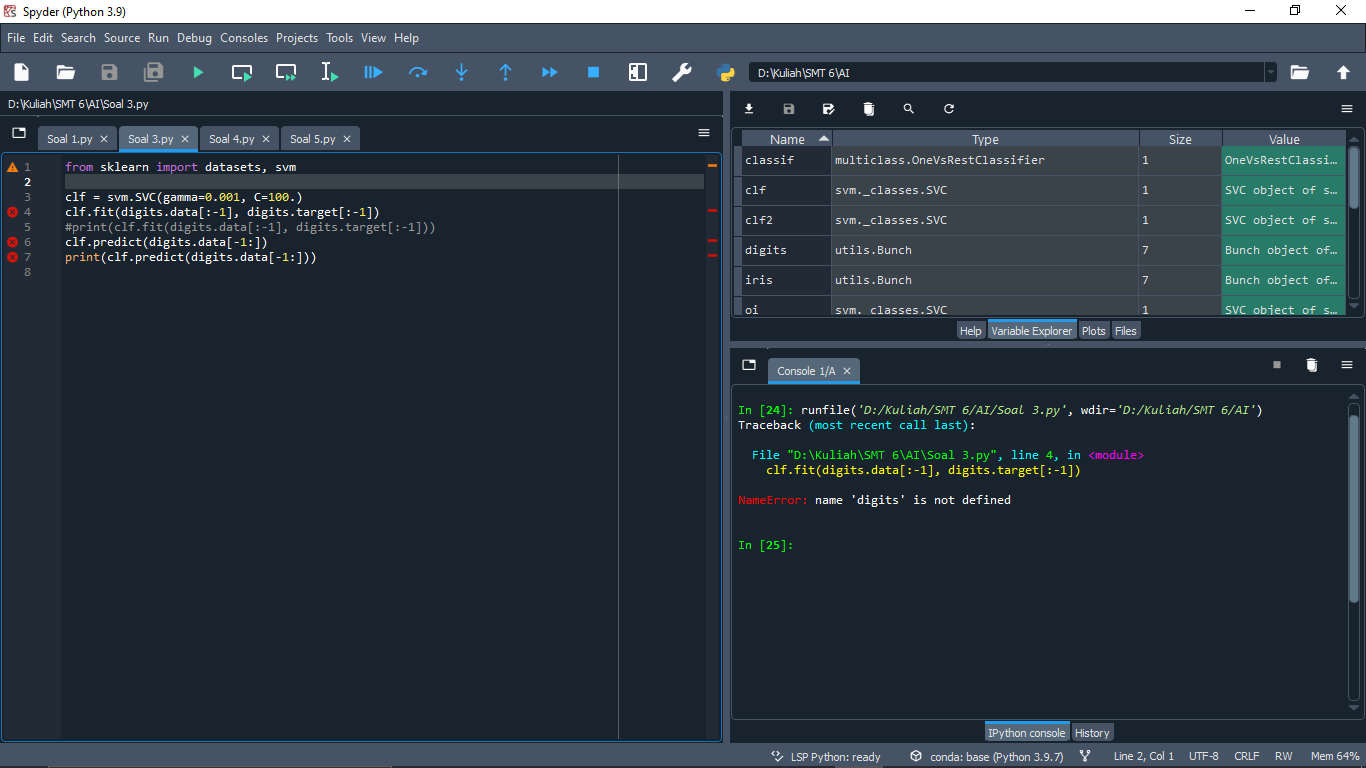
\includegraphics[scale=0.3]{figures/e.1.PNG}
		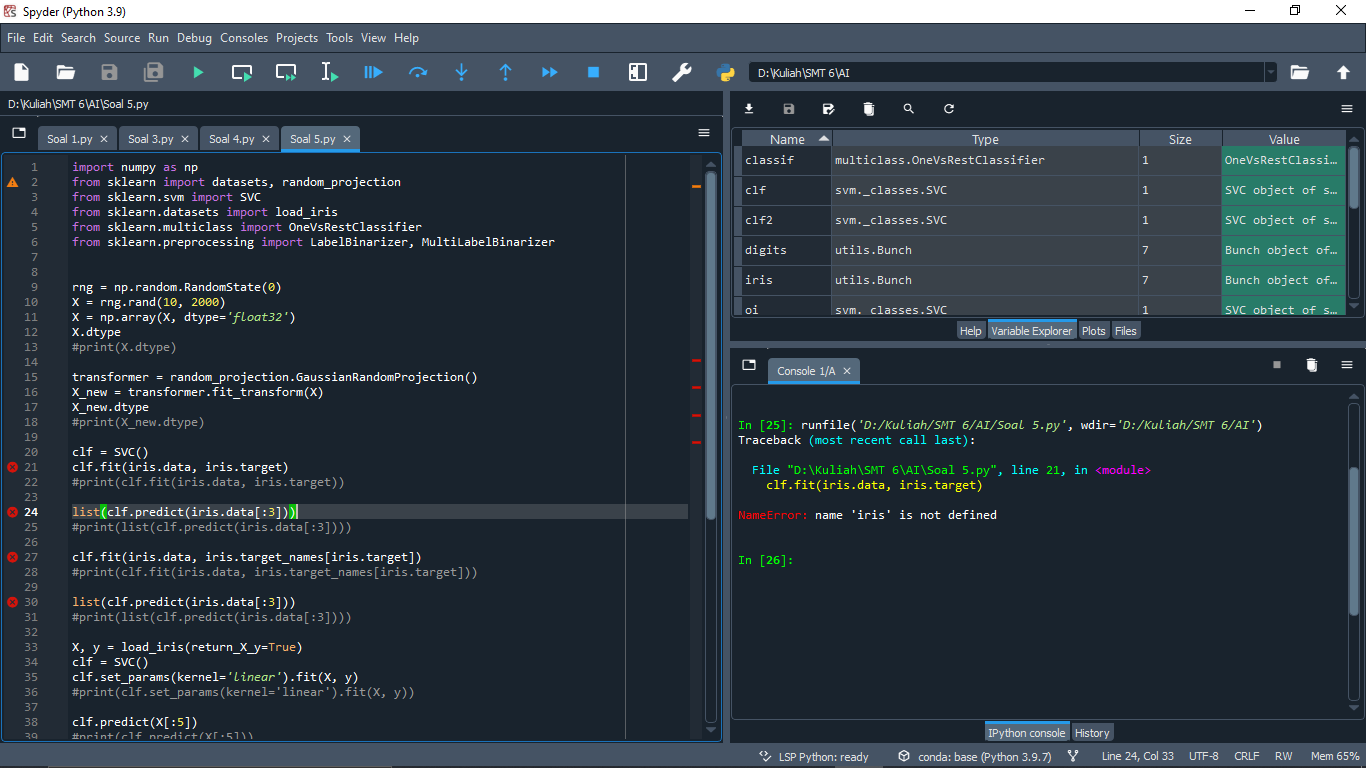
\includegraphics[scale=0.3]{figures/e.2.PNG}
	\end{figure}
	\item
	Tuliskan kode eror dan jenis errornya.
	\begin{enumerate}
		\item NameError: name 'digits' is not defined
		\item NameError: name 'iris' is not defined
	\end{enumerate}
	\item
	Solusi pemecahan masalah error tersebut.
	\begin{enumerate}
		\item NameError = Membuat variabel dengan nama digits yang berisi mengenai dataset dari sklearn.
		\item NameError = Membuat variabel dengan nama iris yang berisi mengenai dataset dari sklearn.
	\end{enumerate}

\end{enumerate}

